\documentclass[tikz,border=2pt]{standalone}
\usepackage{tikz,amsmath}
\usetikzlibrary{arrows.meta, bending,calc,decorations.markings}
\newcommand{\bmR}{\boldsymbol{\mathcal{R}}}
\begin{document}
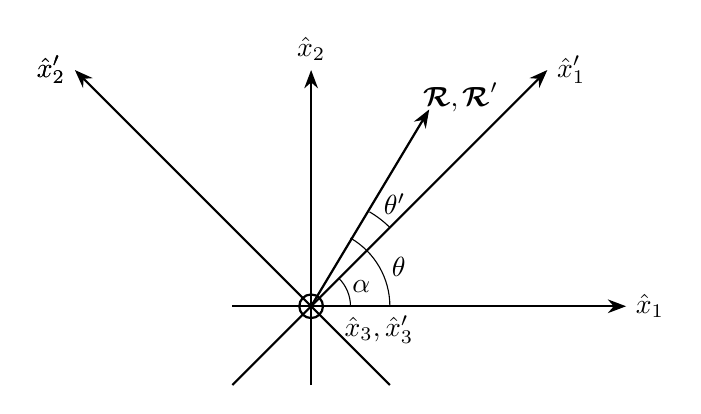
\begin{tikzpicture}[>=Stealth]

\draw [thick,->] (0,-1) -- (5,-1);
\node[right] at (5,-1) {$\hat{x}_1$};
\draw [thick,->](0,-2) -- (4,2);
\node[right] at (4,2) {$\hat{x}_1'$};
\draw [thick,->](1,-2) -- (1,2);
\node[above] at (1,2) {$\hat{x}_2$};
\draw [thick,->](2,-2) -- (-2,2);
\node[left] at (-2,2) {$\hat{x}_2'$};
\draw[thick] (1,-1) circle (0.15cm);
\node[below right] at (1.3,-1) {$\hat{x}_3,\hat{x}_3'$};
\draw [thick,->](1,-1) -- (2.5,1.5);
\node[above right] at (2.3,1.35){$\bmR,\bmR'$};
\node[left] at (-2,2) {$\hat{x}_2'$};

%Angles

\draw (2,-1) arc [start angle=0, end angle=60, radius=1cm];
\node [right] at (1.4,-0.75) {$\alpha$};
\draw (1.5,-1) arc [start angle=0, end angle=45, radius=0.5cm];
\node [right] at (1.9,-0.5) {$\theta$};
\draw (2,0) arc [start angle=45, end angle=60, radius=1.25cm];
\node [right] at (1.8,0.3) {$\theta'$};


\end{tikzpicture}
\end{document}